	\subsection{Pipes} % (fold)
	\label{sub:pipes}
	
		\begin{figure}[ht]
			\caption{Schematische Darstellung einer (unnamed) Pipe}
			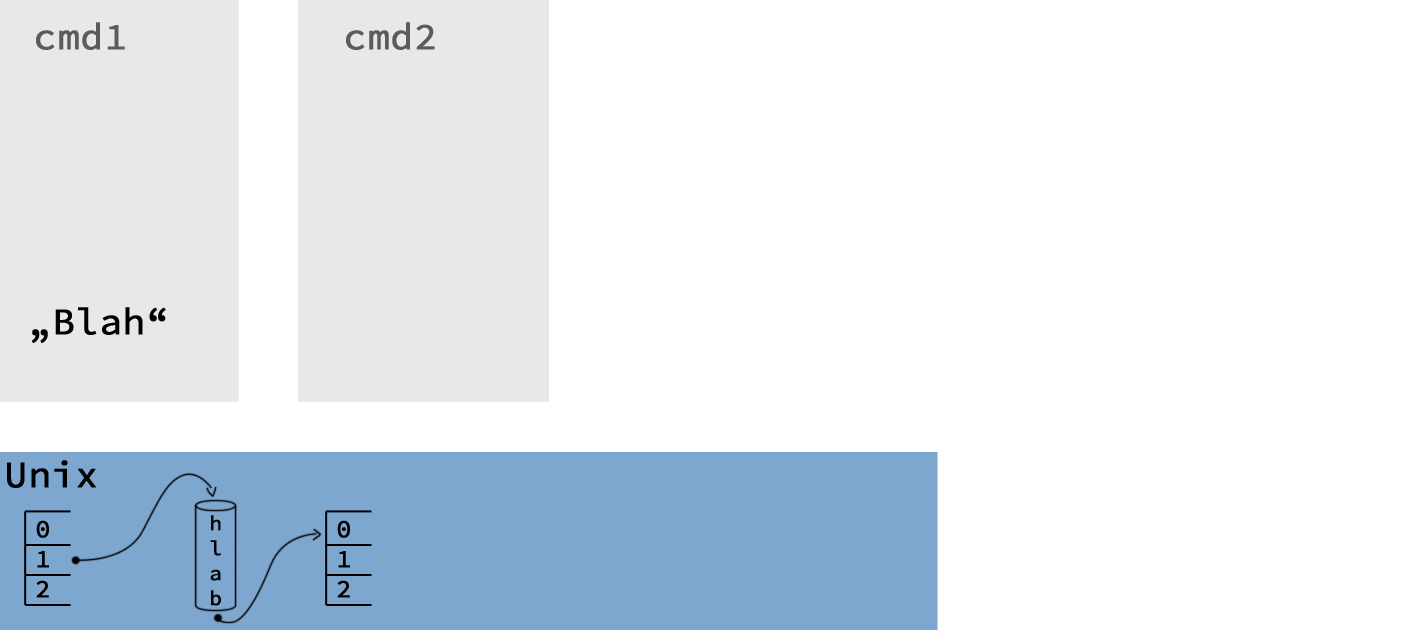
\includegraphics[width=\textwidth]{workfiles/v4_1}
		\end{figure}

		\subsubsection*{Named Pipe} % (fold)
		\label{ssub:named_pipe}

			\lstShell[Variante 1]
			\begin{lstlisting}
cmd filename
cmd2 < filename
			\end{lstlisting}

			\lstShell[Variante 2]
			\begin{lstlisting}
mkfifo filename
cmd filename &
cmd2 < filename
			\end{lstlisting}

		% subsubsection named_pipe (end)

		\subsubsection*{Vorteil Pipes} % (fold)
		\label{ssub:vorteil_pipes}
		
			\begin{itemize}
				\item sequentielle Abarbeitung möglich\\
						(gesamter Datenbestand muss nicht komplett gehalten werden)
				\item 1 arbeitet, 2 muss nicht warten
				\item Prozesssynchronisation\\
						(langsamster Prozess bestimmt die Geschwindigkeit)
			\end{itemize}

		% subsubsection vorteil_pipes (end)

		\subsubsection*{Analog in Haskell} % (fold)
		\label{ssub:analog_in_haskell}
		
			\lstHaskell
			\begin{lstlisting}
head.(map f3).(map f2).(map f1)[1..]
			\end{lstlisting}
(Gibt 1 aus (ohne die gesamten natürlichen Zahlen durchlaufen zu müssen)
		% subsubsection analog_in_haskell (end)

		\subsection*{Interessantes Pipe-Verhalten} % (fold)
		\label{sub:interessantes_pipe_verhalten}
			
			\subsubsection*{cut} % (fold)
			\label{ssub:cut}

				\lstShell
				\begin{lstlisting}
cut -d " " -f 2
				\end{lstlisting}

				Liefertes das f-te Element (\texttt{-f}), Feldtrennung anhand von \texttt{-d}

			% subsubsection cut (end)

			\subsubsection*{tr} % (fold)
			\label{ssub:tr}
			
				\lstShell
				\begin{lstlisting}
tr [:lower:] [:upper:]
				\end{lstlisting}

				Translate übersetzt Zeichen, hier von lower nach upper.

			% subsubsection tr (end)

			\subsubsection*{In Kombination} % (fold)
			\label{ssub:in_kombination}
			
				\lstShell
				\begin{lstlisting}
cut -d " " -f 2 | tr [:lower:] [:upper:]
				\end{lstlisting}

				Läuft nicht wie gewünscht, aber
			
				\lstShell
				\begin{lstlisting}
cut -d " " -f 2 < foo| tr [:lower:] [:upper:]
				\end{lstlisting}

				schon. Was ist das Problem?

				\begin{itemize}
					\item Pufferung im Prozess
					\item wenn FD aus Terminal $\rightarrow$ Zeilenpufferung
					\item wenn FD kein Terminal $\rightarrow$ Blockpufferung (Pipe)
				\end{itemize}

				Lösung daher: Nutzung eines Pseudo-Terminals

				\lstShell
				\begin{lstlisting}
/dev/pty
				\end{lstlisting}

				\begin{figure}[hbtp]
					\caption{pty, Pseudo-Terminal, Schema}
					
\includegraphics[width=\textwidth]{workfiles/v4_2}
				\end{figure}

				\begin{figure}[hbtp]
					
\includegraphics[width=\textwidth]{workfiles/v5_1}
				\end{figure}

				Problem der Blogpufferung: siehe letzte Vorlesung

			% subsubsection in_kombination (end)


	%%%%
	%%%% end V4
	%%%%
	%%%% V5
	%%%%
		% subsection interessantes_pipe_verhalten (end)

		\subsection*{Kommunikation vo Pipes in "`Echtzeit"'} % (fold)
		\label{sub:kommunikation_vo_pipes_in_}

			$\;$
			\begin{figure}[phbt]
				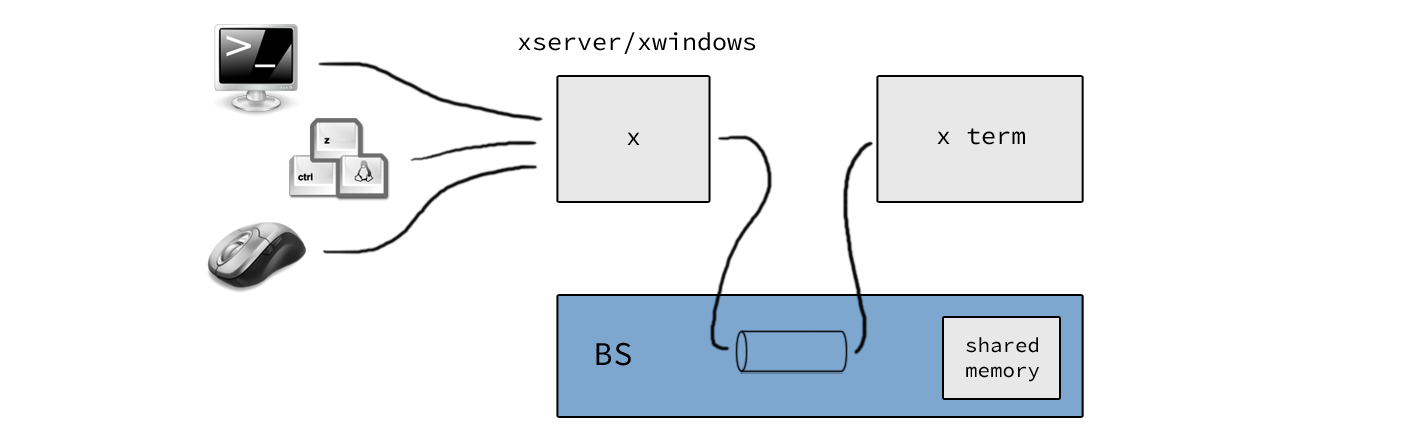
\includegraphics[width=\textwidth]{workfiles/v5_2}
			\end{figure}

			Allerdings keine tatsächliche Echtezit, da unter Unix keine Zeitgarantien exisiteren.
			Harte Echtzeit gibt es bspw. unter OS 9, VxWorks oder PSOS.\\
			Möglich auch durch verteilte Systeme

			\begin{figure}[hbtp]
				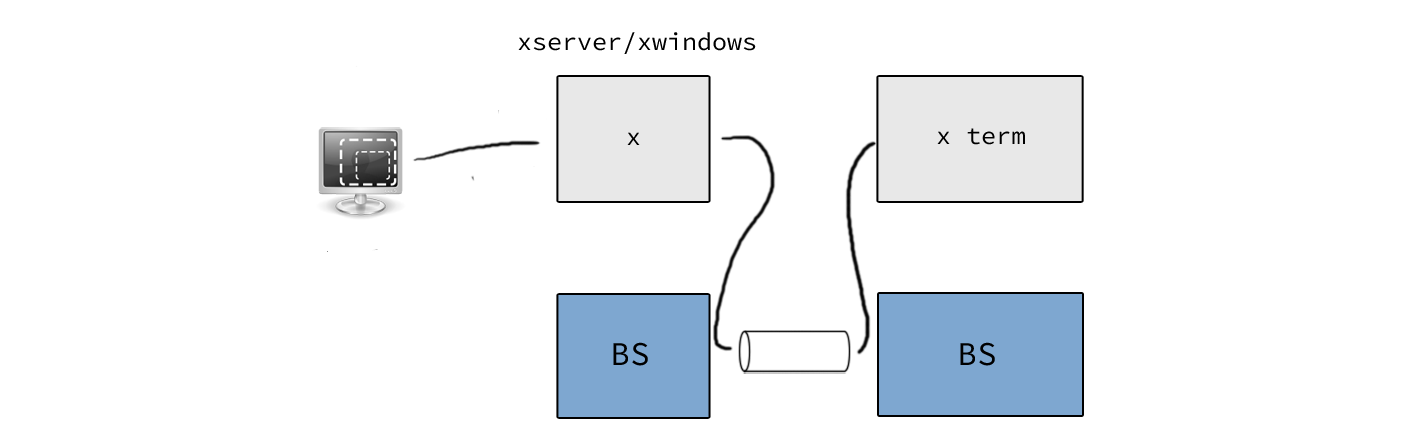
\includegraphics[width=\textwidth]{workfiles/v5_3}
			\end{figure}
		
		% subsection kommunikation_vo_pipes_in_ (end)

	% subsection pipes (end)